\documentclass{article}
\usepackage[margin=0.7in]{geometry}
\usepackage{default}
\usepackage{amsmath,amsthm,amssymb,amsfonts,bm,mathtools,braket,units,array,comment,cases}
\usepackage{fancyhdr,lastpage}
\usepackage{algorithm,algpseudocode}
\usepackage{makecell}
\usepackage[square,numbers]{natbib}
\usepackage{accents}
\usepackage{centernot}
\usepackage{filecontents}
\usepackage{lineno}
\usepackage{tikz}
\usetikzlibrary{matrix}
\usetikzlibrary{shapes.geometric}
\usetikzlibrary{arrows.meta}
\usetikzlibrary{positioning,shapes,arrows}
\usetikzlibrary{calc}
\usetikzlibrary{shapes.multipart}

\def\E{\mathbb{E}}
\def\G{\mathcal{G}}
\def\Pa{\mathrm{Pa}}
\def\R{\mathbb{R}}
\def\Reach{\mathcal{R}}%{\mathrm{Reach}}
\def\Control{\kappa_i}
\def\CL{\mathcal{C}}
\def\OL{\mathcal{O}}
\def\pluseqq{\mathrel{{+}{=}}}
\def\Undirect{\mathcal{U}}%{\mathrm{Undirect}}
\def\qhat{\widehat{q}}
\def\xhat{\widehat{x}}
\def\yhat{\widehat{y}}
\def\zhat{\widehat{z}}
\def\what{\widehat{w}}

\newtheorem{theorem}{Theorem}
\newtheorem{proposition}[theorem]{Proposition}
\newtheorem{lemma}[theorem]{Lemma}
\newtheorem{corollary}[theorem]{Corollary}
\newtheorem{assumption}[theorem]{Assumption}

\linenumbers

\title{Causal inference in neural circuits with open- and closed-loop control}
\author{Adam Willats and Matt O'Shaughnessy}
\date{March 2020}

\bibliographystyle{plainnat}

\begin{document}

\maketitle

\section{Introduction}
\label{sec:introduction}
\subsection{Closed-loop control in neuroscience}
% Takeaways:
% - What is closed-loop control?
% - What does it look like in neuroscience experiments?
% - How does closed-loop control relate to neuroscience identification procedures

\begin{figure}[ht]
	\centering
	 \begin{overpic}[width=.6\textwidth]{figures/figure_sketches/figure1_sketch.png}
	  \end{overpic}
    \caption{\textbf{Text} more text}

    \label{fig:overview} %figure 1
 \end{figure}


\subsection{Interventions from the perspective of causal inference}


\section{Open technical questions}
\label{sec:questions}

\begin{enumerate}
    \item Adam postulates: closed-loop control can act to add a "virtual stimulation" point at an edge where otherwise only recordings are available. This results in off-target / collateral stimulation, but could still allow adding a "open-loop stimulation node" where one could not be physically injected. I think this is worth evaluating as a low-priority theory target
    \item How does "indirect control" (i.e. closed-loop control involving stimulation of one region, and recording from a second, downstream region) fit into this theoretical framework?
\end{enumerate}{}

\section{Identifiability}
\label{sec:identifiability}
\subsection{First thoughts on identifiability}

\paragraph{Initial model.} We begin with the simple linear dynamical system
\begin{equation}
    \begin{cases} \dot{x} = Ax \\ y = Cx + \eta \end{cases}
\end{equation}
where $A$ is the adjacency matrix
\begin{equation}
    \underbrace{\begin{bmatrix} \dot{x}_A \\ \dot{x}_B \\ \dot{x}_C \end{bmatrix}}_{\dot{x}} =
    \underbrace{\begin{bmatrix}
        w_{AA} & w_{AB} & w_{AC} \\
        w_{BA} & w_{BB} & w_{BC} \\
        w_{CA} & w_{CB} & w_{CC}
    \end{bmatrix}}_{A}
    \underbrace{\begin{bmatrix}
        x_A \\
        x_B \\
        x_C
    \end{bmatrix}}_{x}.
    \label{eq:lds}
\end{equation}
Our first question is: What can $A$ tell us about the identifiability of causal relationships between elements of $x$?

\paragraph{Some definitions.}
\begin{enumerate}
    \item Let $\Reach(\cdot) \colon \R^{n \times n} \to \{0,1\}^{n \times n}$ be the operator that maps an adjacency matrix to the binary reachability matrix, in which entry $(i,j)$ is $1$ if $x_i$ is reachable from $x_j$ and $0$ otherwise. In a directed graph, we say that $x_i$ is reachable from $x_j$ if there exists a series of head-to-tail connections from $x_j$ to $x_i$.\footnote{Note that for a binary adjacency matrix $A$, $A^k_{ij} = 1$ $\iff$ $x_i$ is reachable from $x_j$ in $k$ ``hops.'' Using this fact and the fact that $e^A = \sum_{k \geq 0} \tfrac{1}{k!} A^k$, we can compute $\Reach(\cdot)$ as $\Reach(A) = \mathrm{Binarize}(\mathrm{expm}(\mathrm{Binarize}(A)))$.} In an undirected graph, we say that $x_i$ is reachable from $x_j$ if there exists a series of undirected connections from $x_j$ to $x_i$.
    \item Let $\Control \colon \R^{n \times n} \to \R^{n \times n}$ be the operator that applies closed-loop control to fix the output of node $x_i$ regardless of the value of its parents.\footnote{This can be implemented as removing node $i$'s parents, i.e., setting row $i$ of $A$ to zero.}
    \item Let $\Undirect \colon \R^{n \times n} \to \R^{n \times n}$ be the operator that transforms an adjacency matrix to its ``undirected'' equivalent.\footnote{This can be implemented as $\Undirect(A) = (A \neq 0) ~\vert~ (A \neq 0)^T)$ where $\vert$ denotes the element-wise OR operator.}
\end{enumerate}

\paragraph{Supporting observations.}
\begin{enumerate}
    \item The outputs of nodes $i,j$ are uncorrelated if $\Reach(\Undirect(A))_{ij} = 0$.
    \item Closed-loop control ``severs a connection'' if $\Reach(A)_{ij} \neq 0$, but $\Reach(\Control(A))_{ij} = 0$.
\end{enumerate}

\paragraph{Adam's rules of ID.}
\begin{enumerate}  
    \item Two circuits are ``passively ambiguous'' if $\Reach(\Undirect(A)) == \Reach(\Undirect(B))$.
    \item Two circuits are ``open loop ambiguous" if $\Reach(A) == \Reach(B)$.
    \item Two circuits are ``closed loop ambiguous'' \textit{given control at node i} if $\Reach(\Control(A)) == \Reach(\Control(B))$.
    \item Two circuits are ``closed loop ambiguous'' \textit{(given control at any one node)} if $\Reach(\Control(A)) == \Reach(\Control(B))$ for $i = 1, \dots, n$.
\end{enumerate}


\subsection{Background and notation}

\subsubsection{Notation}

We first need to map our notions of ambiguity between circuits to observational and interventional probability distributions. The first step is defining candidate functional circuits as structural causal models (SCMs). Let $\G_1 = (V,E_1)$ and $\G_2 = (V,E_2)$ denote SCMs of two candidate circuits describing the same set of nodes $V$, where $E_1$ and $E_2$ describe the set of edges and functional relationships in each candidate circuit.\footnote{Later we might be able to extend this to the case where there are unobserved nodes affecting the observed nodes.}

We denote the application of closed-loop control to fix a subset of nodes $X \subset V$ to the control signal $x(t)$ by $\CL_{x(t)}(X)$. We denote the application of open-loop control to add the control signal $w(t)$ to the subset of nodes $W \subset V$ by $\OL_{w(t)}(W)$. Recall that (with slight abuse of notation), $E_1$ and $E_2$ denote not only the presence or absence of edges between variables in $V$, but the functional relationships governing these edges. Because knowledge of the SCM $\G$ is equivalent to knowledge of every possible interventional distribution involving variables in $V$, \emph{a functional connection $X \to Y$ is identifiable if and only if we can compute $p(Y \mid \CL_{x(t)}(X))$}.

From a \emph{connection} perspective:
\begin{itemize}
    \item We say that a connection between $X$ and $Y$ ($X, Y \subset V$) is \emph{ambiguous under control scheme $\mathbb{C}$} if there exist multiple causal structures that are consistent with the data collected under $\mathbb{C}$ but have different connections between $X$ and $Y$ (that is, if $\exists$ $\G_1 \neq \G_2$ consistent with the data collected under $\mathbb{C}$ such that $(E_1)_{X,Y} \neq (E_2)_{X,Y}$).
    \item We say that a connection between $X$ and $Y$ is \emph{identifiable under control scheme $\mathbb{C}$} if every casual structure consistent with the data collected under $\mathbb{C}$ has the same causal relationship between $X$ and $Y$ (that is, if $\nexists~ \G_1 \neq \G_2$ such that $\G_1$ and $\G_2$ are both consistent with the data collected under $\mathbb{C}$ but $(E_1)_{X,Y} \neq (E_2)_{X,Y}$).
\end{itemize}

From a \emph{whole circuit} perspective:
\begin{itemize}
    \item We say that a circuit is \emph{ambiguous under control scheme $\mathbb{C}$} if there exist multiple causal structures that are consistent with the data collected under the control scheme but that have different edge sets (that is, if $\exists$ $\G_1 \neq \G_2$ consistent with the data collected under $\mathbb{C}$).
    \item We say that a circuit is \emph{identifiable under control scheme $\mathbb{C}$} if there is only one possible causal structure consistent with the data collected using the control scheme (that is, if $\nexists$ $\G_1 \neq \G_2$ consistent with the data collected under $\mathbb{C}$).
\end{itemize}
%More mathematically, let $\mathbb{C} = \left(X, w(t), C\right)_{i}$, $i = 1, \dots$, represent a control scheme consisting of (1) a set of nodes $X \subset V$ that control is applied to, (2) a control signal $w(t) \in \R$ ($t \geq 0$) that is used for control of $X$, and (3) the method of control $C \in \{\OL,\CL\}$ (open- or closed-loop). If $C = \OL$, then application of control fixes $X(t) \leftarrow X(t) + w(t)$; if $C = \CL$, then application of control fixes $X(t) \leftarrow w(t)$. Further let $p_{\mathbb{C}}(V)$ denote the joint distribution over $V$ under application of control scheme $\mathbb{C}$. (Todo: continue here.)

\subsubsection{Do-calculus}

The do-calculus tells us when and how we can compute interventional distributions from observational data. Our goal is to extend this result to control, including the possibility of open loop (i.e., imperfect) interventions.

\begin{theorem}[Rules of $do$-calculus]
    \label{thm:do-calculus}
    Let $\G$ be a directed acyclic graph associated with a causal model inducing probability distributions $p(\cdot)$. Define $\G_{\underline{X}}$ to be the causal graph with connections leaving $X$ removed, and $\G_{\overline{X}}$ to be the causal graph with connections entering $X$ removed. Then for any disjoint subsets of variables $X, Y, Z, W$:
    \begin{enumerate}
        \item (Insertion/deletion of observations) $p(y \mid do(x), z, w) = p(y \mid do(x), w)$ if $Y \perp Z \mid X, W$ in $\G_{\overline{X}}$.
        \item (Action/observation exchange) $p(y \mid do(x), do(z), w) = p(y \mid do(x), z, w)$ if $Y \perp Z \mid X, W$ in $\G_{\overline{X},\underline{Z}}$.
        \item (Insertion/deletion of actions) $p(y \mid do(x), do(z), w) = p(y \mid do(x), w)$ if $Y \perp Z \mid X, W$ in $\G_{\overline{X},\overline{Z(W)}}$, where $Z(W)$ is the set of nodes that are not ancestors of any node in $W$ in $\G_{\overline{X}}$.
    \end{enumerate}
\end{theorem}

\begin{proof} The following proofs can be found in the appendix of \cite{pearl1995causal}:
    \begin{enumerate}
        \item Intervening on $X$ in $\G$ produces the modified graph $\G_{\overline{X}}$, the graph with arrows entering $X$ removed. Since by assumption $Y \perp Z \mid X, W$ in this modified graph, we have the conditional independence statement $p(y \mid do(x), z, w) = p(y \mid do(x), w)$.
        \item Intervening on $X$ in $\G$ produces the modified graph $\G_{\overline{X}}$, and the assumption $Y \perp Z \mid X, W$ in $\G_{\overline{X},\underline{Z}}$ therefore guarantees that all backdoor paths from $Z$ to $Y$ in $\G_{\overline{X}}$ are blocked\footnote{A backdoor path from $Z$ to $Y$ is which the arrow connected to $Z$ \emph{enters} $Z$.}. The effect on $Y$ of conditioning and intervening on $Z$ are therefore the same.
        \item todo
    \end{enumerate}
\end{proof}

\begin{theorem}[Completeness of the $do$-calculus (todo-citation)]
    \label{thm:do-calculus-completeness}
    The $do$-calculus is complete. That is, a quantity $p(y \mid do(x), z)$ is identifiable (from observational data\footnote{Todo: work through proof of this fact using open/closed loop control}) if and only if it can be reduced to a $do$-free expression using the $do$-calculus.
\end{theorem}

\begin{corollary}[Identifiability of neural circuits using control]
    The connection $X \to Y$ is identifiable under closed-loop control scheme $\mathbb{C}$ if and only if $p(y \mid do(x))$ can be computed from the distributions induced by $\mathbb{C}$ using the rules of Theorem \ref{thm:do-calculus}.
\end{corollary}

\subsection{Identifiability with closed-loop control}

What causal relationships in a graph are identifiable when closed-loop control is applied to certain nodes? Here we approach this question by deriving a form of the do-calculus to the linear dynamical system \eqref{eq:lds}.

\subsection{Identifiability with open-loop control}
\begin{figure}
    \centering
    \begin{tabular}{ccc}
        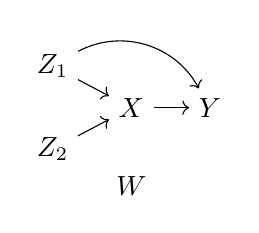
\begin{tikzpicture}
            \node (X) {$X$};
            \node[right of=X] (Y) {$Y$};
            \node[left of=X, yshift=+1.5em] (Z1) {$Z_1$};
            \node[left of=X, yshift=-1.5em] (Z2) {$Z_2$};
            \node[below of=X] (W) {$W$};
    	    \path[->] (Z1) edge (X);
    	    \path[->] (Z2) edge (X);
    	    %\path[->] (W) edge (X);
    	    \path[->] (X) edge (Y);
    	    \path[->, bend left=45] (Z1) edge (Y);
    	\end{tikzpicture} \qquad & \qquad
    	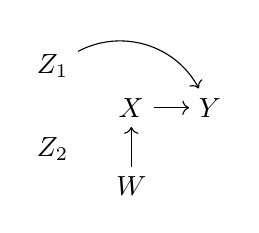
\begin{tikzpicture}
    	    \node (X) {$X$};
            \node[right of=X] (Y) {$Y$};
            \node[left of=X, yshift=+1.5em] (Z1) {$Z_1$};
            \node[left of=X, yshift=-1.5em] (Z2) {$Z_2$};
            \node[below of=X] (W) {$W$};
    	    %\path[->] (Z1) edge (X);
    	    %\path[->] (Z2) edge (X);
    	    \path[->] (W) edge (X);
    	    \path[->] (X) edge (Y);
    	    \path[->, bend left=45] (Z1) edge (Y);
	    \end{tikzpicture} \qquad & \qquad
	    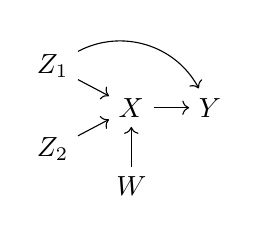
\begin{tikzpicture}
            \node (X) {$X$};
            \node[right of=X] (Y) {$Y$};
            \node[left of=X, yshift=+1.5em] (Z1) {$Z_1$};
            \node[left of=X, yshift=-1.5em] (Z2) {$Z_2$};
            \node[below of=X] (W) {$W$};
    	    \path[->] (Z1) edge (X);
    	    \path[->] (Z2) edge (X);
    	    \path[->] (W) edge (X);
    	    \path[->] (X) edge (Y);
    	    \path[->, bend left=45] (Z1) edge (Y);
	    \end{tikzpicture} \\~\\
	    (a) Original circuit \qquad & \qquad (b) CL control \qquad & \qquad (c) OL control
	\end{tabular}
	\caption{Modifications of circuit to represent closed- and open-loop control. $Z_1$ denotes nodes that are parents of both $X$ and $Y$; $Z_2$ denotes nodes that are parents of $X$ but not $Y$.}
    \label{fig:effective-dags-after-control}
\end{figure}

In \cite[Ch.~4.2]{pearl2009causality}, Pearl proposes an identification framework for a broader class of interventions that can be described as $x \coloneqq g(z)$, where $g$ is some (potentially stochastic) function depending on a separate set of nodes $z$. The effect on $Y$ of an intervention on $X$ that depends on another set of nodes\footnote{This must be true in an acyclic graph because $Z \to X$. However, this non-descendants assumption does not necessarily hold in presence of feedback, in which case the analysis in this section breaks down.} $W$ is
\begin{align}
    p(y \mid do(x=g(w))) &= \int_w p(y \mid do(x=g(w)), w) p(w \mid do(x=g(w))) dw \qquad \text{(marginalization)} \\
    &= \int_w p(y \mid do(x=g(w)), w) p(w) dw \qquad \text{($W \notin \mathrm{De}(X)$)} \\
    &= \E_{w} \left[ p(y \mid do(x=g(w)), w) \right].
\end{align}

Therefore, \emph{we can determine the causal influence of $x$ on $y$, $p(y \mid \widehat{x})$, if we can obtain $p(y \mid \widehat{x}, w)$ and $p(w)$ using measurements from our control scheme}.

To see how we can apply this framework to our model, denote $Z \coloneqq \mathrm{Pa}(X)$, and represent the (open- or closed-loop) control input by $W$. Compared to the original circuit (Figure \ref{fig:effective-dags-after-control}a), applying closed-loop control replaces the causal link(s) $Z \to X$ with $W \to X$ (Figure \ref{fig:effective-dags-after-control}b), while applying open-loop control simply adds the causal link $W \to X$ (Figure \ref{fig:effective-dags-after-control}c).

Applying similar analysis to our model of \emph{closed-loop control} (Figure \ref{fig:effective-dags-after-control}(b)) yields
\begin{align}
    p(y \mid do(x = W)) &= \int_w \int_{z_2} p(y \mid do(x = W), W, z_2) p(W, z_2 \mid do(x = W)) dw dz_2 \qquad \text{(marginalization)} \\
    &= \int_w \int_{z_2} p(y \mid do(x=W), W, z_2) p(W,z_2) dw dz_2 \qquad \text{($W,Z_2 \notin De(X)$)} \\
    &= \int_w \int_{z_2} p(y \mid do(x=W), W, z_2) p(W) p(z_2) dw dz_2 \qquad \text{($W \perp Z_2$)} \\
    &= \int_{z_2} p(y \mid do(x=W), z_2) p(z_2) dz_2 \qquad \text{($p(W) = \delta_{W=W}$)} \\
    &= \E_{z_2} \left[ p(y \mid do(x=W), z_2) \right].
\end{align}
Therefore, \emph{we can determine the causal influence of $x$ on $y$, $p(y \mid \widehat{x})$, if we can obtain $p(y \mid \widehat{x}, z_2)$ and $p(z_2)$}.

Applying similar analysis to our model of \emph{open-loop control} (Figure \ref{fig:effective-dags-after-control}(c)) yields
\begin{align}
    p(y \mid do(x = f(z) + W)) &= \int_w \int_z p(y \mid do(x = f(z) + W), W, z) p(W, z \mid do(x=f(z)+W)) dw dz \\
    &= \int_w \int_z p(y \mid do(x = f(z) + W), W, z) p(W, z) dw dz \\
    &= \int_w \int_z p(y \mid do(x = f(z) + W), W, z) p(W) p(z) dw dz \\
    &= \int_z p(y \mid do(x = f(w) + \what), \what, w) p(w) dw \qquad \text{(since $p(W) = \delta_{W=\what}$)} \\
    &= \E_w \left[ p(y \mid do(x=f(w)+\what), w) \right].
\end{align}
This relationship tells us that applying open-loop control tells us something less than $p(y \vert \xhat)$.

Todo --- read:
\begin{itemize}
    \item Pearl, ``A probabilistic calculus of actions,'' Proc.\ UAI 1994.
    \item Kuroki and Miyakawa, ``Covariate selection for estimating the causal effect of control plans using causal diagrams,'' J.\ Royal Stat.\ Soc.\ Ser.\ B, 2003.
\end{itemize}

\section{Examples}
\label{sec:examples}
\begin{figure}[h]
    \centering
    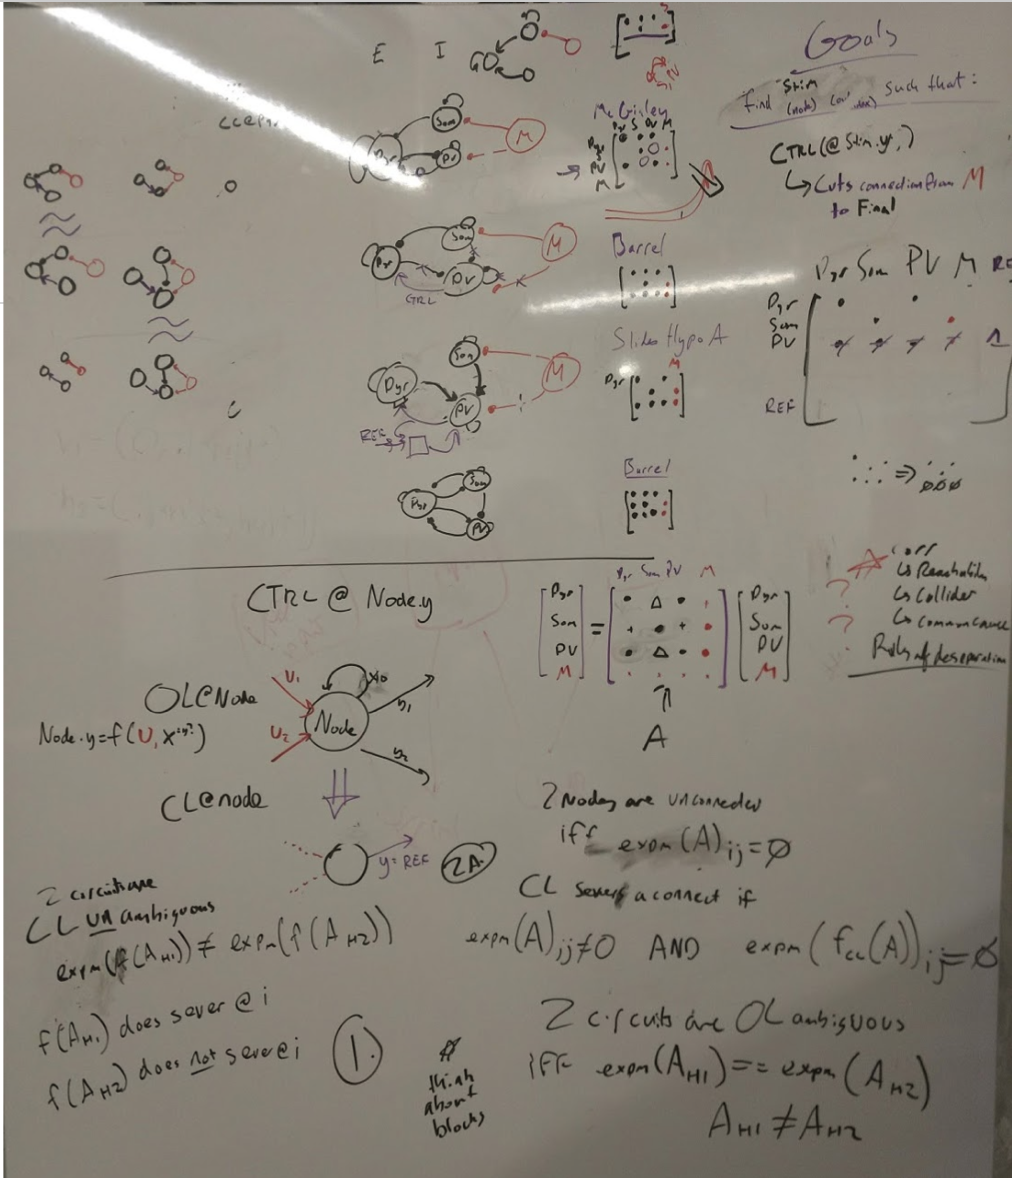
\includegraphics[width=\textwidth]{big_circuit_wb.png}
    \caption{Circuit diagrams}
\end{figure}

\begin{figure}[h]
    \centering
    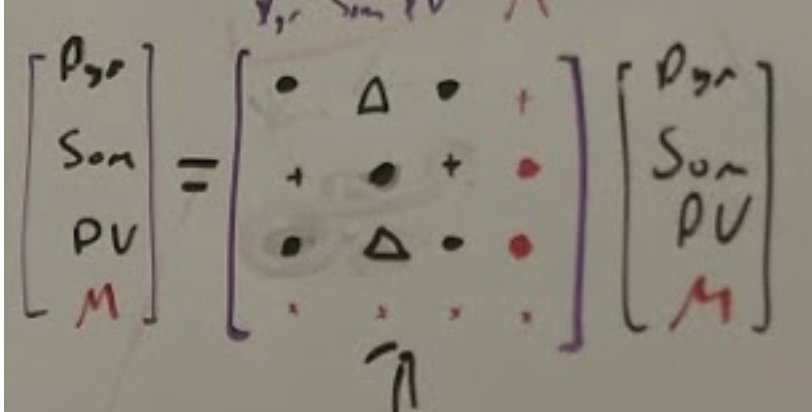
\includegraphics[width=\textwidth]{just_adj_mat.png}
    \caption{Linear representation of functional model}
\end{figure}

\begin{figure}[h]
    \centering
    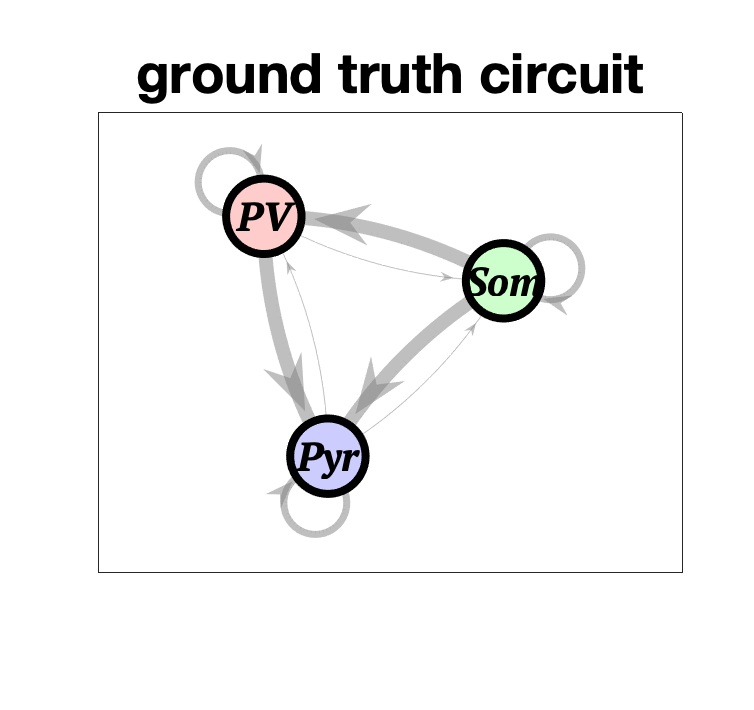
\includegraphics[width=\textwidth/2]{obsv_graph.png}
    \caption{graph representation of cortical circuit}
\end{figure}

\begin{figure}[h]
    \centering
    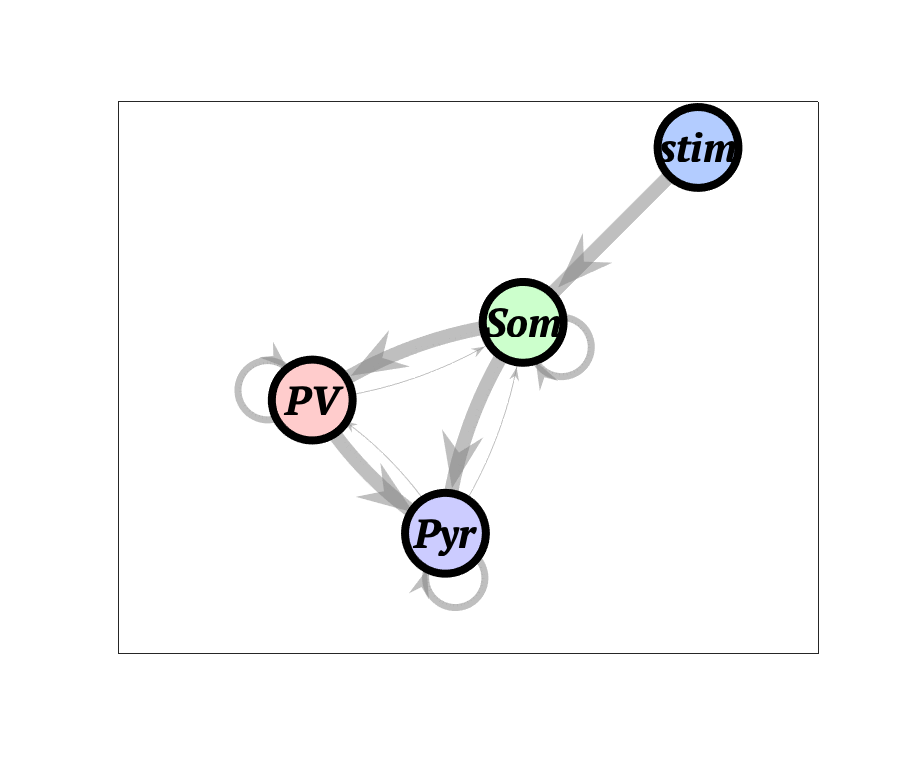
\includegraphics[width=\textwidth/2]{ol_graph.png}
    \caption{graph representation of open-loop control applied to cortical circuit}
\end{figure}

\begin{figure}[h]
    \centering
    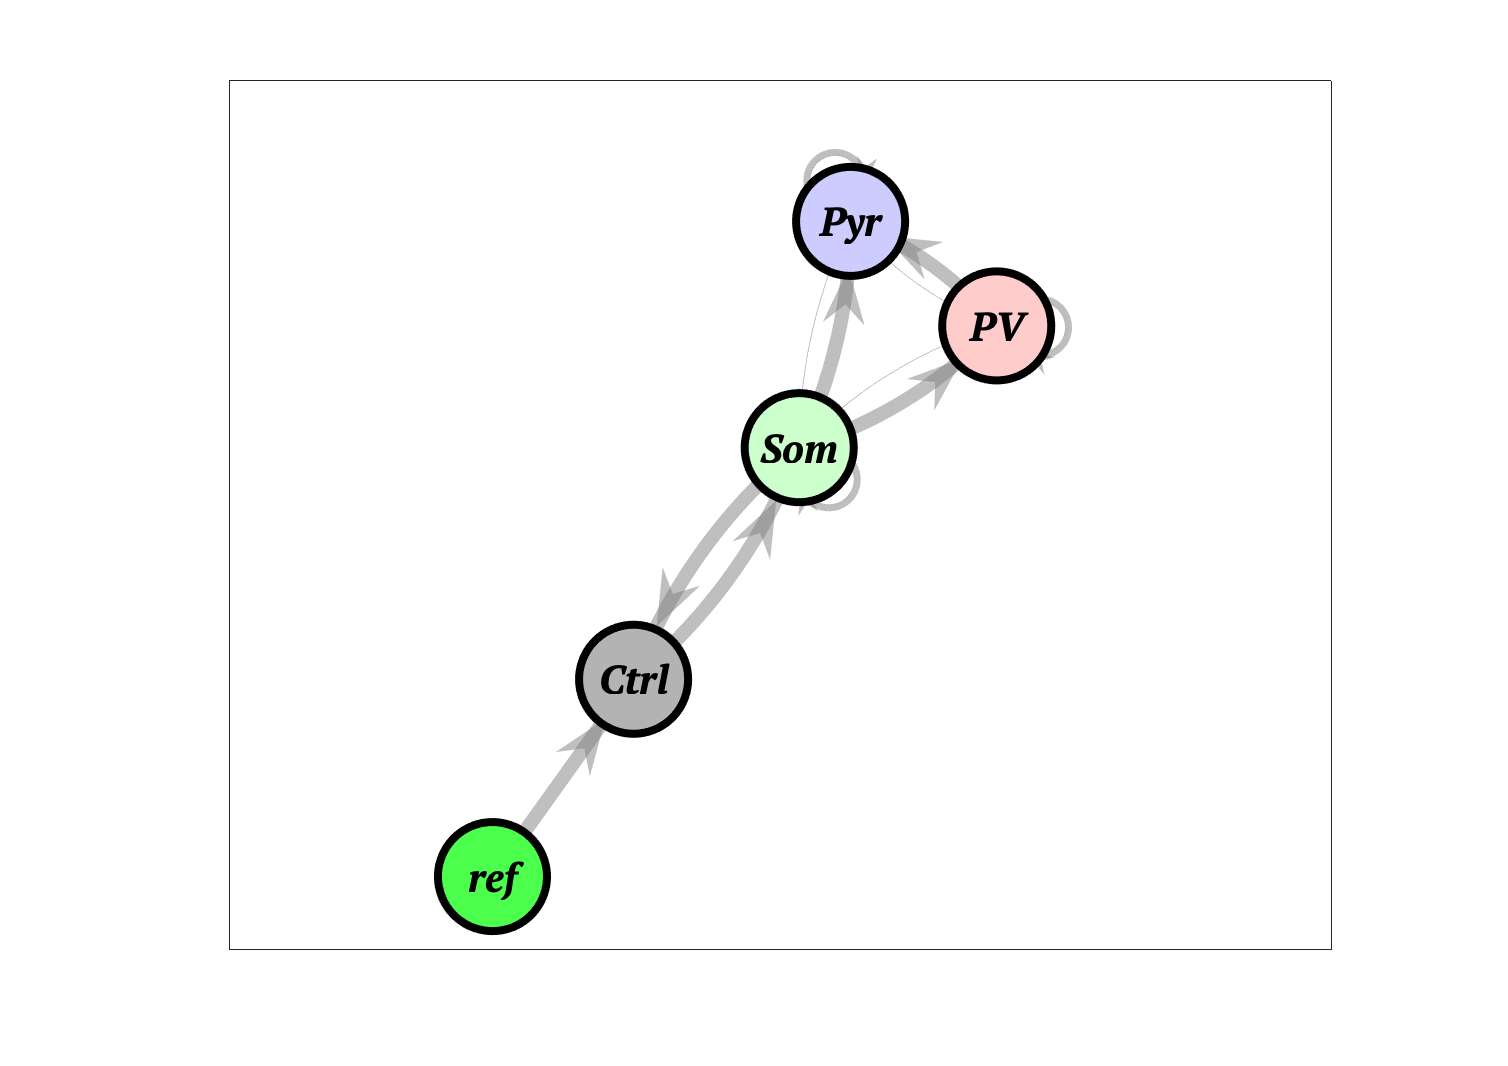
\includegraphics[width=\textwidth/2]{cl_graph.png}
    \caption{graph representation of closed-loop control applied to cortical circuit}
\end{figure}

\begin{table}[h!]
    \centering
    \begin{tabular}{|c|c|c|c|c|c|}
     \hline
     \begin{bmatrix}
     1 & 1 & 1\\
     0 & 1 & 0\\
     1 & 0 & 1
     \end{bmatrix}
      & 
     \begin{bmatrix}
     1 & 1 & 1\\
     1 & 1 & 0\\
     1 & 0 & 1
     \end{bmatrix}
      & 
     \begin{bmatrix}
     1 & 1 & 1\\
     0 & 1 & 0\\
     0 & 0 & 0
     \end{bmatrix}
      & 
     \begin{bmatrix}
     1 & 1 & 1\\
     0 & 1 & 0\\
     1 & 1 & 1
     \end{bmatrix}
      & 
     \begin{bmatrix}
     1 & 1 & 1\\
     1 & 1 & 1\\
     1 & 1 & 1
     \end{bmatrix}
      & 
     \begin{bmatrix}
     1 & 1 & 1\\
     0 & 1 & 0\\
     0 & 0 & 1
     \end{bmatrix}
     
     \\ \hline
     \begin{bmatrix}
     1 & 1 & 1\\
     0 & 1 & 0\\
     1 & 1 & 1
     \end{bmatrix}
      & 
     \begin{bmatrix}
     1 & 1 & 1\\
     1 & 1 & 1\\
     1 & 1 & 1
     \end{bmatrix}
      & 
     \begin{bmatrix}
     1 & 1 & 1\\
     0 & 1 & 0\\
     0 & 0 & 0
     \end{bmatrix}
      & 
     \begin{bmatrix}
     1 & 1 & 1\\
     0 & 1 & 0\\
     1 & 1 & 1
     \end{bmatrix}
      & 
     \begin{bmatrix}
     1 & 1 & 1\\
     1 & 1 & 1\\
     1 & 1 & 1
     \end{bmatrix}
      & 
     \begin{bmatrix}
     1 & 1 & 1\\
     0 & 1 & 0\\
     0 & 0 & 1
     \end{bmatrix}
     
     \\ \hline
     \begin{bmatrix}
     1 & 0 & 1\\
     0 & 1 & 0\\
     1 & 1 & 1
     \end{bmatrix}
      & 
     \begin{bmatrix}
     1 & 0 & 1\\
     0 & 1 & 1\\
     1 & 1 & 1
     \end{bmatrix}
      & 
     \begin{bmatrix}
     1 & 0 & 1\\
     0 & 1 & 0\\
     0 & 0 & 0
     \end{bmatrix}
      & 
     \begin{bmatrix}
     1 & 1 & 1\\
     0 & 1 & 0\\
     1 & 1 & 1
     \end{bmatrix}
      & 
     \begin{bmatrix}
     1 & 1 & 1\\
     1 & 1 & 1\\
     1 & 1 & 1
     \end{bmatrix}
      & 
     \begin{bmatrix}
     1 & 0 & 1\\
     0 & 1 & 0\\
     0 & 0 & 1
     \end{bmatrix}
     
     \\ \hline
     \begin{bmatrix}
     1 & 1 & 1\\
     1 & 1 & 0\\
     1 & 1 & 1
     \end{bmatrix}
      & 
     \begin{bmatrix}
     1 & 1 & 1\\
     1 & 1 & 1\\
     1 & 1 & 1
     \end{bmatrix}
      & 
     \begin{bmatrix}
     1 & 1 & 1\\
     1 & 1 & 0\\
     0 & 0 & 0
     \end{bmatrix}
      & 
     \begin{bmatrix}
     1 & 1 & 1\\
     1 & 1 & 1\\
     1 & 1 & 1
     \end{bmatrix}
      & 
     \begin{bmatrix}
     1 & 1 & 1\\
     1 & 1 & 1\\
     1 & 1 & 1
     \end{bmatrix}
      & 
     \begin{bmatrix}
     1 & 1 & 1\\
     1 & 1 & 1\\
     0 & 0 & 1
     \end{bmatrix} \\
     \hline
     \end{tabular}
     
     \caption{Adjacency matrices for examples of passive and open-loop ambiguous circuits.}
\end{table}

\hrulefill \\
\paragraph{Dynamics equations for various models}
PLDS, SISO:
\begin{flalign}
& x = \begin{bmatrix}
    x_A \\
    x_B \\
    x_C
    \end{bmatrix} &\\
& \dot{x} = Ax + Q\omega &\\
& y = Cx + \eta &\\
& z = \exp(y) &\\
& spk = \mathrm{Poiss}(z) & 
\end{flalign}

\hrulefill \\
PLDS, SISO w/Inputs:
\begin{flalign}
& x = \begin{bmatrix}
    x_A \\
    x_B \\
    x_C
    \end{bmatrix} &\\
& \dot{x} = Ax + Q\omega + Bu&\\
& y = Cx + \eta &\\
& z = \exp(y) &\\
& spk = \mathrm{Poiss}(z) & 
\end{flalign}

\hrulefill \\
Network of PLDS, MIMO:

\bibliography{moshaughnessy.bib}

\end{document}
    